\documentclass{article}
\usepackage[utf8]{inputenc}
\usepackage{amsmath}
\usepackage{amssymb}
\usepackage{amsthm}
\usepackage{cancel}
\usepackage[shortlabels]{enumitem}
\usepackage{caption}
\usepackage{graphicx}
\usepackage[top=0.5in, bottom=0.5in, left=1in, right=1in]{geometry}

% \usepackage{titlesec}
%     \titlespacing{\subsection}{\parindent}{15pt}{12pt}

\title{\textbf{\underline{MATH3090U: Netwrok Science}\\Assignment 2}}
\author{Syed Naqvi\\100590852}
\date{\today}

\begin{document}

    \maketitle

    \subsection*{1.}    
    
    \vspace*{10pt}
    \begin{enumerate}[label=(\alph*), left=10pt, itemsep=10pt]
        
        \item \begin{minipage}[t]{0.9\textwidth}
                The shortest path between nodes 1 and 7 is the path $[1,3,6,7]$.
                The reason why this is the shortest path is because it contains a number of edges that
                is less than or equal to the number of edges contained in all other paths from nodes
                1 to 7.
            \end{minipage}
        
        \item \begin{minipage}[t]{0.9\textwidth}
                The diameter of G is 4 because out of all distances between two
                nodes that exist in G, 4 is the maximum.
            \end{minipage}
        
        \item \begin{minipage}[t]{0.9\textwidth}
                The length of the longest simple cycle (circumference) of G
                is 4. This is because there exists no sequence beginning
                and ending at the same node (closed walk), that also
                doesnt repeat any vertices except the first and last and is longer than length 4. 
            \end{minipage}

        \item \begin{minipage}[t]{0.9\textwidth}
                A bridge in graph G is defined as an edge $\{u,v\}$ such that $G-\{u,v\}$ is
                disconnected. Thus the only bridges in this graph are edges $\{8, 9\}$ and
                $\{8, 10\}$ since removing them disconnects nodes 9 and 10 from the rest of
                the graph. All other edges lie on cycles and so cannot be bridges since their
                adjacent nodes will remain connected by a path other than the removed edge.
            \end{minipage}

        \item \begin{minipage}[t]{0.9\textwidth}
                The closeness centrality of node 3 can be calculated as follows:
                \begin{align*}
                    C_{3}   &=  \frac{n-1}{\sum_{j\neq i}^{} dist(i,j)}\\
                    C_{3}   &=  \frac{9}{\sum_{j\neq 3}^{} dist(3,j)}\\
                            &=  \frac{9}{dist(3,1) + dist(3,2) + dist(3,4) + dist(3,5) +
                                dist(3,6) + dist(3,7) + dist(3,8) + dist(3,9) + dist(3,10)}\\
                            &=  \frac{9}{1+1+1+1+1+2+2+3+3}\\
                            &= \frac{9}{15}\\
                            &= \frac{3}{5}
                \end{align*}
                $\therefore$ the closesness centrality of node 3 is $\displaystyle \frac{3}{5}$.
            \end{minipage}
    
        \newpage
    
        \item \begin{minipage}[t]{0.9\textwidth}
                The betweenness centrality of node 5 is calculated as follows:
                \begin{align*}
                    b_{5}   &= \sum_{\substack{s,t\\s\neq t\neq i}} \frac{\sigma_{s,t}(i)}{\sigma_{s,t}}\\
                            &= \frac{\sigma_{1,2}(5)}{\sigma_{1,2}}
                               + \frac{\sigma_{1,3}(5)}{\sigma_{1,3}}
                               + \frac{\sigma_{1,4}(5)}{\sigma_{1,4}}
                               + \frac{\sigma_{1,6}(5)}{\sigma_{1,6}}
                               + \frac{\sigma_{1,7}(5)}{\sigma_{1,7}}
                               + \frac{\sigma_{1,8}(5)}{\sigma_{1,8}}
                               + \frac{\sigma_{1,9}(5)}{\sigma_{1,9}}
                               + \frac{\sigma_{1,10}(5)}{\sigma_{1,10}}\\
                            &+   \frac{\sigma_{2,3}(5)}{\sigma_{2,3}}
                               + \frac{\sigma_{2,4}(5)}{\sigma_{2,4}}
                               + \frac{\sigma_{2,6}(5)}{\sigma_{2,6}}
                               + \frac{\sigma_{2,7}(5)}{\sigma_{2,7}}
                               + \frac{\sigma_{2,8}(5)}{\sigma_{2,8}}
                               + \frac{\sigma_{2,9}(5)}{\sigma_{2,9}}
                               + \frac{\sigma_{2,10}(5)}{\sigma_{2,10}}\\
                            &+   \frac{\sigma_{3,4}(5)}{\sigma_{3,4}}
                               + \frac{\sigma_{3,6}(5)}{\sigma_{3,6}}
                               + \frac{\sigma_{3,7}(5)}{\sigma_{3,7}}
                               + \frac{\sigma_{3,8}(5)}{\sigma_{3,8}}
                               + \frac{\sigma_{3,9}(5)}{\sigma_{3,9}}
                               + \frac{\sigma_{3,10}(5)}{\sigma_{3,10}}\\
                            &+   \frac{\sigma_{4,6}(5)}{\sigma_{4,6}}
                               + \frac{\sigma_{4,7}(5)}{\sigma_{4,7}}
                               + \frac{\sigma_{4,8}(5)}{\sigma_{4,8}}
                               + \frac{\sigma_{4,9}(5)}{\sigma_{4,9}}
                               + \frac{\sigma_{4,10}(5)}{\sigma_{4,10}}\\
                            &+   \frac{\sigma_{6,7}(5)}{\sigma_{6,7}}
                               + \frac{\sigma_{6,8}(5)}{\sigma_{6,8}}
                               + \frac{\sigma_{6,9}(5)}{\sigma_{6,9}}
                               + \frac{\sigma_{6,10}(5)}{\sigma_{6,10}}\\
                            &+   \frac{\sigma_{7,8}(5)}{\sigma_{7,8}}
                               + \frac{\sigma_{7,9}(5)}{\sigma_{7,9}}
                               + \frac{\sigma_{7,10}(5)}{\sigma_{7,10}}\\
                            &+   \frac{\sigma_{8,9}(5)}{\sigma_{8,9}}
                               + \frac{\sigma_{8,10}(5)}{\sigma_{8,10}}\\
                            &+   \frac{\sigma_{9,10}(5)}{\sigma_{9,10}}\\
                            &=   \frac{0}{1}
                               + \frac{0}{1}
                               + \frac{0}{1}
                               + \frac{0}{1}
                               + \frac{0}{1}
                               + \frac{0}{1}
                               + \frac{0}{1}
                               + \frac{0}{1}\\
                            &  + \frac{0}{1}
                               + \frac{0}{1}
                               + \frac{0}{1}
                               + \frac{0}{1}
                               + \frac{0}{1}
                               + \frac{0}{1}
                               + \frac{0}{1}\\
                            &  + \frac{0}{1}
                               + \frac{0}{1}
                               + \frac{0}{1}
                               + \frac{0}{1}
                               + \frac{0}{1}
                               + \frac{0}{1}\\
                            &  + \frac{0}{1}
                               + \frac{0}{1}
                               + \frac{0}{1}
                               + \frac{0}{1}
                               + \frac{0}{1}\\
                            &  + \frac{0}{1}
                               + \frac{0}{1}
                               + \frac{0}{1}
                               + \frac{0}{1}\\
                            &  + \frac{0}{1}
                               + \frac{0}{1}
                               + \frac{0}{1}\\
                            &  + \frac{0}{1}
                               + \frac{0}{1}\\
                            &  + \frac{0}{1}\\
                            &=0
                \end{align*}
                $\therefore$ the betweenness centrality of node 5 is $0$.\\\\
                This answer makes sense because for all pairs of nodes in the graph where node 5 is not
                one of the nodes in the pair, any shortest path between the nodes does not include node 5.

            \end{minipage}
        
        \item \begin{minipage}[t]{0.9\textwidth}
                Yes, nodes 1, 2, 4, 7, 9, 10 also have betweenness centralities of 0. This makes sense
                because just like node 5, each of these nodes also does not lie on any shortest path
                between any two other nodes in the graph.
            \end{minipage}
        
        \item \begin{minipage}[t]{0.9\textwidth}
                This is \textbf{True}.\\
                If we consider a node where all pairs of its adjacent nodes are connected then this node
                will have local clustering coefficient of 1. This also means that the shortest path
                from any of this node's neighbours to any other neighbour will always be 1 since they are all
                adjacent. It follows then that the betweenness centrality of the original node
                will be zero since it cannot lie on the shortest path between any pair of its neighbours. 
            \end{minipage}

    \end{enumerate}

    \newpage

    \subsection*{2.}    
    
    \vspace*{10pt}
    \begin{enumerate}[label=(\alph*), left=10pt, itemsep=10pt]
        \item \begin{minipage}[t]{0.9\textwidth}
                To find the transitivity of graph \(G\) in question 1, we first find its adjacency matrix
                \(A\) as well as \(A^{2}\) and \(A^{3}\).
                
                \vspace{2em}  % add some space for better formatting
                
                \begin{minipage}{0.5\linewidth}
                    \textbf{Matrix \(A\):}
                    \[
                    \left[
                    \begin{matrix}
                        0 & 1 & 1 & 1 & 0 & 0 & 0 & 0 & 0 & 0\\
                        1 & 0 & 1 & 1 & 0 & 0 & 0 & 0 & 0 & 0\\
                        1 & 1 & 0 & 1 & 1 & 1 & 0 & 0 & 0 & 0\\
                        1 & 1 & 1 & 0 & 0 & 0 & 0 & 0 & 0 & 0\\
                        0 & 0 & 1 & 0 & 0 & 1 & 0 & 0 & 0 & 0\\
                        0 & 0 & 1 & 0 & 1 & 0 & 1 & 1 & 0 & 0\\
                        0 & 0 & 0 & 0 & 0 & 1 & 0 & 1 & 0 & 0\\
                        0 & 0 & 0 & 0 & 0 & 1 & 1 & 0 & 1 & 1\\
                        0 & 0 & 0 & 0 & 0 & 0 & 0 & 1 & 0 & 0\\
                        0 & 0 & 0 & 0 & 0 & 0 & 0 & 1 & 0 & 0\\
                    \end{matrix}
                    \right]
                    \]
                \end{minipage}\hfill
                \begin{minipage}{0.5\linewidth}
                    \textbf{Matrix \(A^{2}\):}
                    \[
                    \left[
                    \begin{matrix}
                        3 & 2 & 2 & 2 & 1 & 1 & 0 & 0 & 0 & 0\\
                        2 & 3 & 2 & 2 & 1 & 1 & 0 & 0 & 0 & 0\\
                        2 & 2 & 5 & 2 & 1 & 1 & 1 & 1 & 0 & 0\\
                        2 & 2 & 2 & 3 & 1 & 1 & 0 & 0 & 0 & 0\\
                        1 & 1 & 1 & 1 & 2 & 1 & 1 & 1 & 0 & 0\\
                        1 & 1 & 1 & 1 & 1 & 4 & 1 & 1 & 1 & 1\\
                        0 & 0 & 1 & 0 & 1 & 1 & 2 & 1 & 1 & 1\\
                        0 & 0 & 1 & 0 & 1 & 1 & 1 & 4 & 0 & 0\\
                        0 & 0 & 0 & 0 & 0 & 1 & 1 & 0 & 1 & 1\\
                        0 & 0 & 0 & 0 & 0 & 1 & 1 & 0 & 1 & 1\\
                    \end{matrix}
                    \right]
                    \]
                \end{minipage}

                \vspace{1em}  % add some space for better formatting

                \begin{minipage}{0.5\linewidth}
                    \textbf{Matrix \(A^{3}\):}
                    \[
                    \left[
                    \begin{matrix}
                        6 & 7 & 9 & 7 & 3 & 3 & 1 & 1 & 0 & 0\\
                        7 & 6 & 9 & 7 & 3 & 3 & 1 & 1 & 0 & 0\\
                        9 & 9 & 8 & 9 & 6 & 8 & 2 & 2 & 1 & 1\\
                        7 & 7 & 9 & 6 & 3 & 3 & 1 & 1 & 0 & 0\\
                        3 & 3 & 6 & 3 & 2 & 5 & 2 & 2 & 1 & 1\\
                        3 & 3 & 8 & 3 & 5 & 4 & 5 & 7 & 1 & 1\\
                        1 & 1 & 2 & 1 & 2 & 5 & 2 & 5 & 1 & 1\\
                        1 & 1 & 2 & 1 & 2 & 7 & 5 & 2 & 4 & 4\\
                        0 & 0 & 1 & 0 & 1 & 1 & 1 & 4 & 0 & 0\\
                        0 & 0 & 1 & 0 & 1 & 1 & 1 & 4 & 0 & 0\\
                    \end{matrix}
                    \right]
                    \]
                \end{minipage}

                \vspace{2em}

                Each entry $(i,j)$ of $A^{2}$ where $i \neq j$ is the number of simple paths of length two from
                node $i$ to node $j$ in graph $G$. Hence, the sum of all off-diagnoal entries in $A^{2}$ counts
                the total number of simple paths of length two in $G$ (here $i \rightarrow k \rightarrow j$ and 
                $j \rightarrow k \rightarrow i$ are different paths). Since A is an adjacency matrix for a simple
                undirected graph, we know that A will be symmetric, and because $(A^{2})^{T} = (AA)^{T} = A^{T}
                A^{T} = AA = A^{2}$, $A^{2}$ is also symmetric. Since $A^{2}$ is symmetric, we know that the sum
                of all off-diagonal entries is the same as the sum of all entries above or below the main diagonal
                times 2.\\

                Thus the total number of simple paths of length two in G is
                $\displaystyle 2\sum_{i>j}\left(A^{2}\right)_{ij}$.\\

                The trace of $A^{3}$ counts the number of simple cycles of length three in G.\\

                We can now calculate the transitivity of G:
                \begin{align*}
                    t(G) &= \frac{\text{number of simple cycles of length three in graph G}}{\text{number of simple paths of length two in G}}\\
                         &= \frac{trace(A^{3})}{2\displaystyle\sum_{i>j}^{}\left(A^{2}\right)_{ij}}\\
                         &= \frac{36}{2(33)}\\
                         &= 0.5454\overline{54}
                \end{align*}
                $\therefore$ the transitivity of the graph in question 1 is $t(G) = 0.5454\overline{54}$
            \end{minipage}
            \newpage

        \item \begin{minipage}[t]{0.9\textwidth}
                $t(G)$ is equal to 1 only for complete graphs on $n$ vertices. In such graphs, every
                2-length simple path must necessarily be part of a closed triangle due to all nodes
                being connected. Furthermore, all closed triangles have the same number of 3-length simple
                cycles as they do 2-length simple paths. Thus for each additional
                2-length simple path, we add one simple 3-length cycle and so the numerator and
                denominator of the transitivity fraction will always be the same for complete graphs
                on $n$ nodes.  
            \end{minipage}

        \addtocounter{enumi}{1}
        \item \begin{minipage}[t]{0.9\textwidth}
                For directed graph D, we count the number of edges and cycles of length two
                directly.
                \begin{align*}
                    r(D) &= \frac{\text{cycles of length two}}{\text{number of edges in }D}\\
                        &= \frac{8}{13}
                \end{align*}
                $\therefore$ the reciprocity of D is $\displaystyle\frac{8}{13}$.
            \end{minipage}

        \item \begin{minipage}[t]{0.9\textwidth}
                The graph from part (c) is strongly connected because for all nodes
                $u,v \in V(D)$ where $u \neq v$, there is a directed path from $u$ to $v$
                and from $v$ to $u$.
            \end{minipage}

        \item \begin{minipage}[t]{0.9\textwidth}
            This is \textbf{True}.\\
            If $D$ is weakly connected, then there exists a path $P$ for all nodes
            $u,v \in V(D)$ where $u \neq v$ such that, ignoring edge direction, $P$
            connects $u$ and $v$. Consider now that $r(D) = 1$, this implies that for all
            $u,v \in V(D)$ s.t. $(u,v) \in E(D)$, it must also be the case that
            $(v,u) \in E(D)$ meaning that all exsiting edges in $D$ have a reciprocal edge.
            Thus, each directed edge in $P$ must have a reciprocal edge allowing us to follow
            $P$ as a directed path from $u$ to $v$ as well as a directed path from $v$ to $u$.
            Since $u$ and $v$ are arbitrary, $D$ is strongly connected.\\

            $\therefore$ if $D$ is weakly-connected and $r(D)=1$, then $D$ must also be
            strongly connected.
        
        \end{minipage}

        \item \begin{minipage}[t]{0.9\textwidth}
            Let $B$ be the adjacency matrix of an arbitrary directed graph $D$.
            We note that even though $D$ is a directed graph, each entry $(i,j)$ in matrix
            $B^{2}$ still represents the number of walks of length 2 from node $i$ to node $j$.
            This is because every entry $(i,k)$ in row $i$ of $B$ is the number of directed edges
            from node $i$ to node $k$ and each entry $(k,j)$ in column $j$ of $B$ is the number of
            directed edges from node $k$ to node $j$. When we find entry $(i,j)$ in $B^{2}$
            we are calculating the sum $\sum_{k=1}^{n}(B)_{ik}(B)_{k,j}$ which is
            only incrememented when there exist paths from $i$ to $k$ and from $k$ to $j$,
            resutlting in entry $(i,j)$ of $B^{2}$ consisting of the number of walks of length 2
            from node $i$ to node $j$.\\\\
            Following this logic we see that values in entry $(i,i)$ of $B^{2}$ are the
            number of ways to get from node $i$ back to itself. This counts the number of cycles
            of length 2 that $i$ is a part of, meaning that $trace(B^{2})$ is the total number
            of cycles of length 2 in graph $D$, where $i\rightarrow k \rightarrow i$ and
            $k \rightarrow i \rightarrow k$ count as two different cycles. Since the trace
            of a matrix is equal to the sum of its eigenvalues, and if matrix $B$ has
            eigenvalues $\lambda_{1}, \lambda_{2}, \dots \lambda_{n}$ then matrix $B^{2}$ has
            eigenvalues $\lambda^{2}_{1}, \lambda^{2}_{2}, \dots \lambda^{2}_{n}$ and
            $trace(B^{2}) = \lambda^{2}_{1}+\lambda^{2}_{2}+ \dots +\lambda^{2}_{n}$.\\\\
            If $m$ is the total number of edges in $D$ then we can write an expression for
            $r(D)$ as follows:
            \begin{align*}
                r(D) &= \frac{\text{number of cycles of length two}}{\text{number of edges in }D}\\
                     &= \frac{trace(B^{2})}{m}\\
                     &= \frac{(\lambda^{2}_{1}+\lambda^{2}_{2}+ \dots +\lambda^{2}_{n})}{m}
            \end{align*}
            $\therefore$ an expression for $r(D)$ in terms of $m$ and the eigenvalues of the
            adjacency matrix of $D$ is
            $\displaystyle\frac{(\lambda^{2}_{1}+\lambda^{2}_{2}+ \dots +\lambda^{2}_{n})}{m}$.
        \end{minipage}
    \end{enumerate}
    
    \subsection*{3.}
    \vspace*{10pt}
    \begin{enumerate}[label=(\alph*), left=10pt, itemsep=10pt]
        \item \begin{minipage}[t]{0.9\textwidth}
            For any tree with $n$ vertices, there are $n-1$ edges. If we let $L$ be the number
            of leaves then $L$ is also the total degree of all leaves since each leaf has
            degree 1. We can let $I$ be the total number of internal nodes and $I_{deg}$ be
            the total internal degree. Remembering that the total graph degree is 2 times
            the number of edges, we can express $n$ and $n-1$ as follows:
            \begin{equation}
                |V(T)| = n = L + I
            \end{equation}
            \begin{equation}
                |E(T)| = n-1 = \frac{L+I_{deg}}{2}
            \end{equation}
            We know that tree $T$ in our case has 50 leaves and an equal number, $x$, of internal
            nodes with degrees 2,3,4 and 5. Thus the total internal degree will always be
            $I_{deg}=x(2+3+4+5)=14x$ while the total number of internal nodes will always be
            $I=4x$. Based on this information we can substitute, solve for $x$ and then find $n$:
            \begin{align*}
                |V(T)|-1  &= |E(T)|\\
                n-1       &= \frac{L+I_{deg}}{2}\\
                (L + I)-1 &= \frac{L+I_{deg}}{2}\\
                (50+4x)-1 &= \frac{50 + 14x}{2}\\
                100+8x-2  &= 50+14x\\
                48        &= 6x\\
                x         &= 8
            \end{align*}
            solving for $n$ we get:
            \begin{align*}
                n &= 50 + 4(8)\\
                n &= 82
            \end{align*}
            $\therefore$ $T$ has 82 vertices.

        \end{minipage}
    \end{enumerate}

    \vspace{1em}

    \subsection*{4.}
    \vspace*{10pt}
    \begin{enumerate}[label=(\alph*), left=10pt, itemsep=10pt]
        \item \begin{minipage}[t]{0.9\textwidth}
            My process for finding a minimum spanning tree is to scan the graph and choose a
            cycle at random. I then remove the highest weighted edge from the cycle and then
            select another cycle at random. I repeat this process until i arrive at a minimum
            spanning tree. This approach ensures that out of all edges whose removal would
            not disconnect the graph, only the highest weighted are removed.\\

            \textbf{Minimum Spanning Tree}\\
                \begin{minipage}[t]{0.9\textwidth}
                    \vspace{0.1em} % some vertical space after the caption   
                    \centering
                    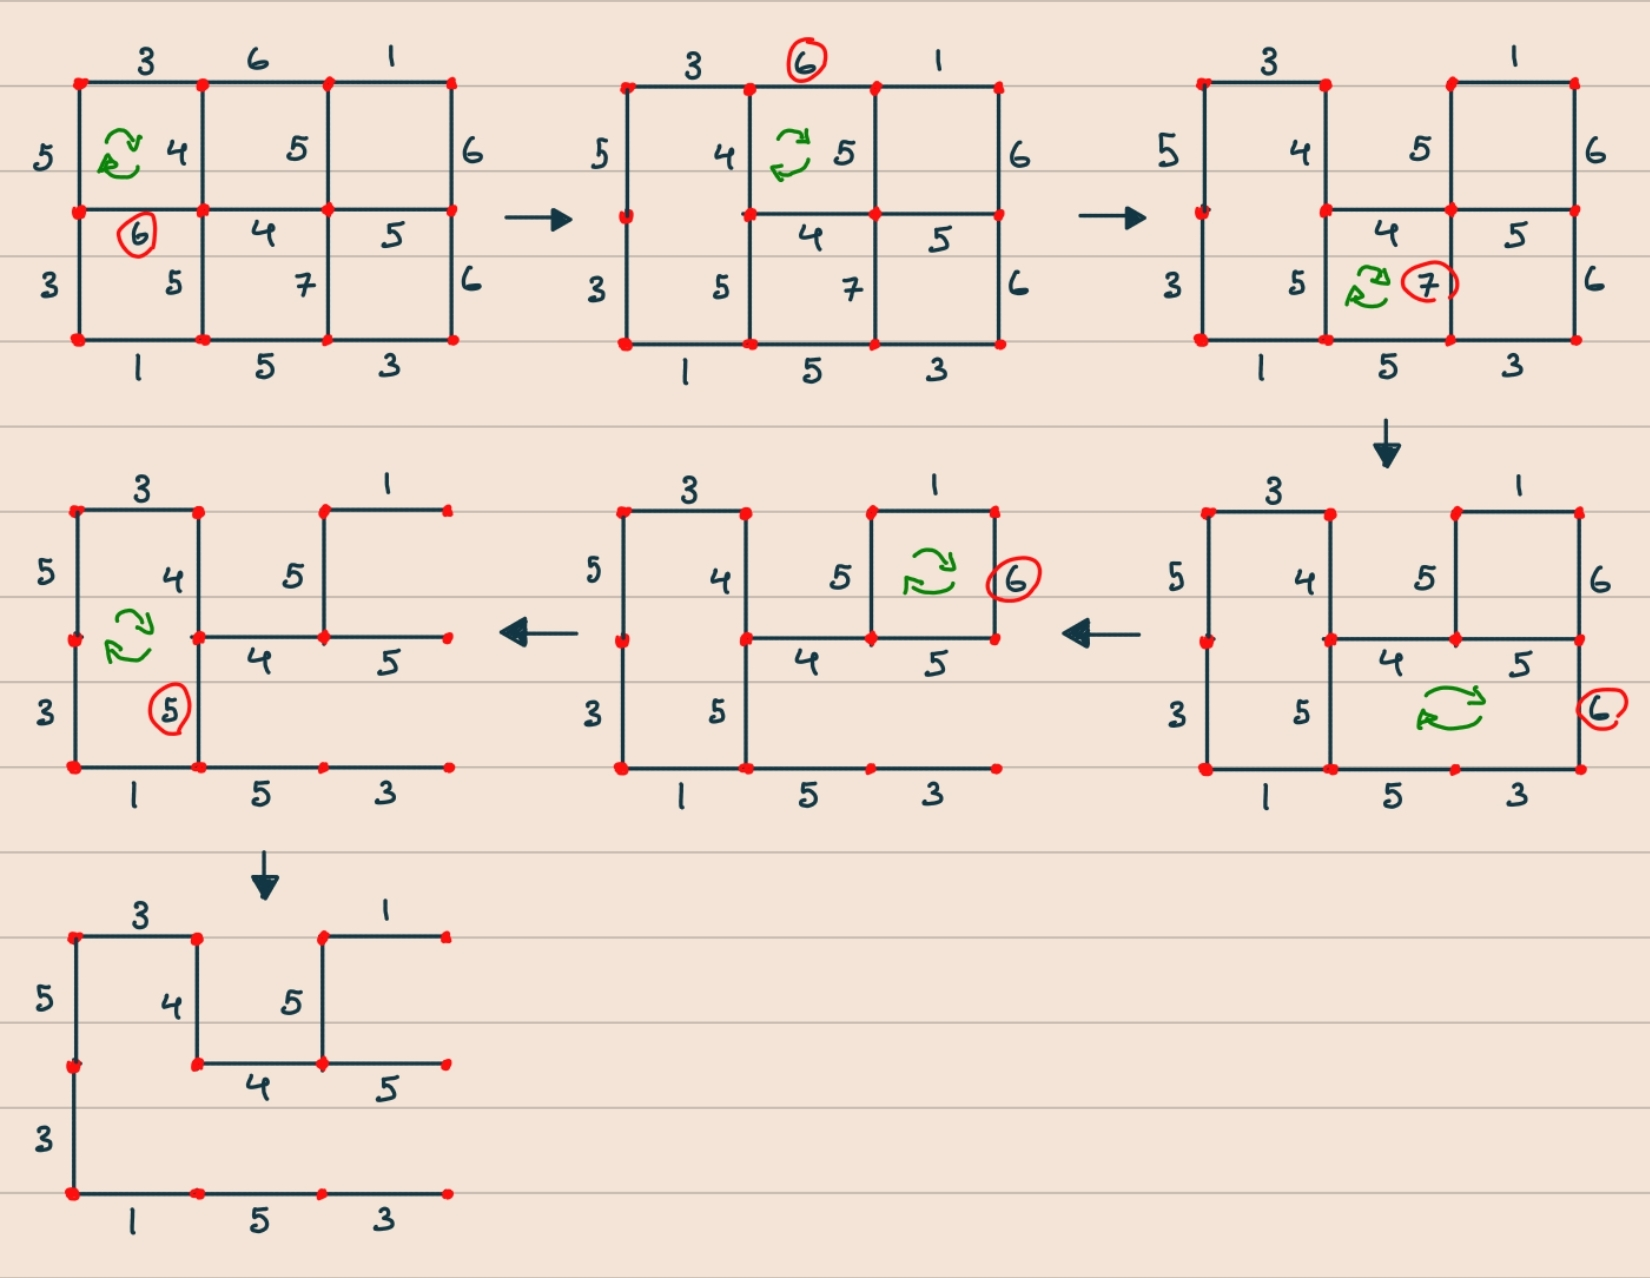
\includegraphics[width=5.9in]{./4a.jpg} 
                \end{minipage}
        \end{minipage}

        \item \begin{minipage}[t]{0.9\textwidth}
            The minimum spanning tree for an arbitrary weighted undirected graph is not unique
            in general. Take the case where there are multiple edges of the same weight in a
            single cycle. Removing any such edge results in the same final weight but not
            necessarily the same final graph.\\

            We can illustrate by presenting two different minimum spanning trees of the
            graph in the previous question:\\

            \textbf{Multiple Minimum Spanning Trees}\\
                \begin{minipage}[t]{0.9\textwidth}
                    \vspace{0.1em} % some vertical space after the caption   
                    \centering
                    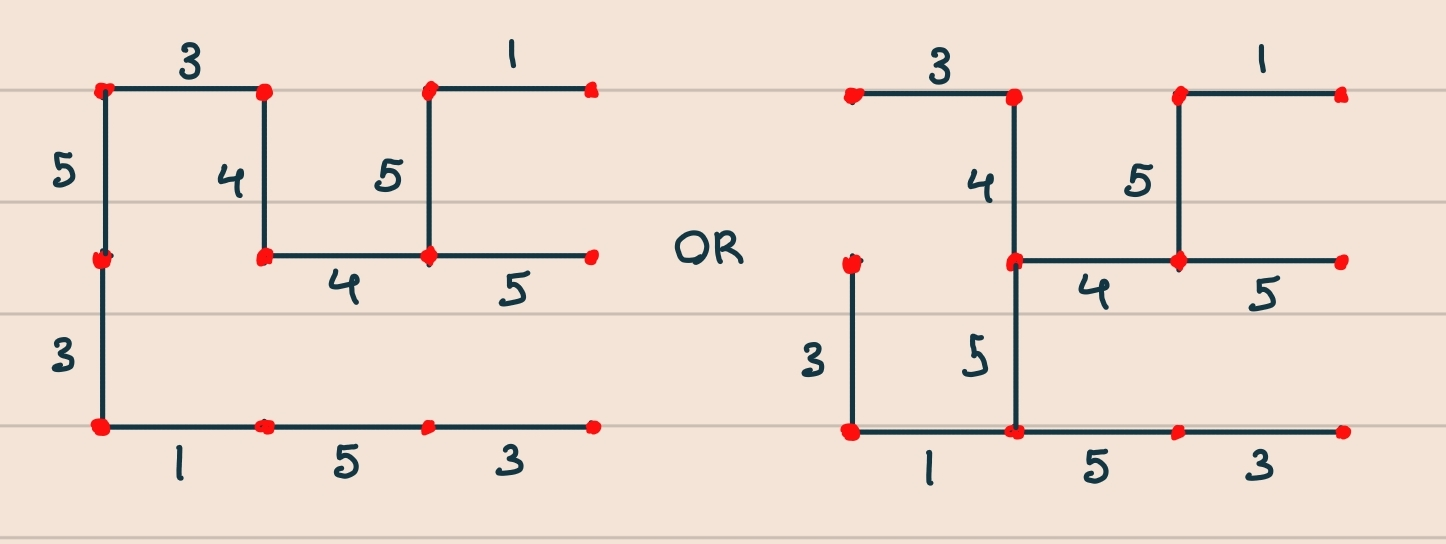
\includegraphics[width=5.9in]{./4b.jpg} 
                \end{minipage}
        \end{minipage}

        \item \begin{minipage}[t]{0.9\textwidth}
            This is \textbf{False}.\\
            Counting the $n-1$ smallest edge weights arbitrarily does not gurantee the weight
            of a minimum spanning tree for the graph. This is due to the possibility of bridges
            whose weights may not fall within the $n-1$ smallest, but must be included in the
            count since their removal would disconnect the graph and by definition, minimum
            spanning trees are both connected and spanning.
        \end{minipage}
    \end{enumerate}
    \vspace{1em}
    \subsection*{5.}
    \vspace*{10pt}
    \begin{enumerate}[label=(\alph*), left=10pt, itemsep=10pt]
        \item \begin{minipage}[t]{0.9\textwidth}
                \begin{minipage}[t]{0.9\textwidth}
                    \vspace{0.1em} % some vertical space after the caption   
                    \centering
                    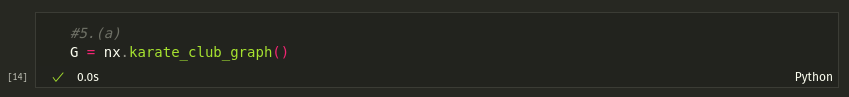
\includegraphics[width=5.9in]{./5a.png} 
                \end{minipage}
        \end{minipage}
        \item \begin{minipage}[t]{0.9\textwidth}
            \begin{minipage}[t]{0.9\textwidth}
                \vspace{0.1em} % some vertical space after the caption   
                \centering
                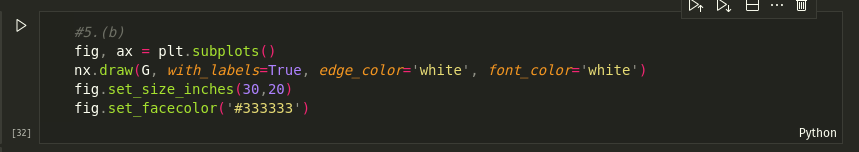
\includegraphics[width=5.9in]{./5bi.png}
                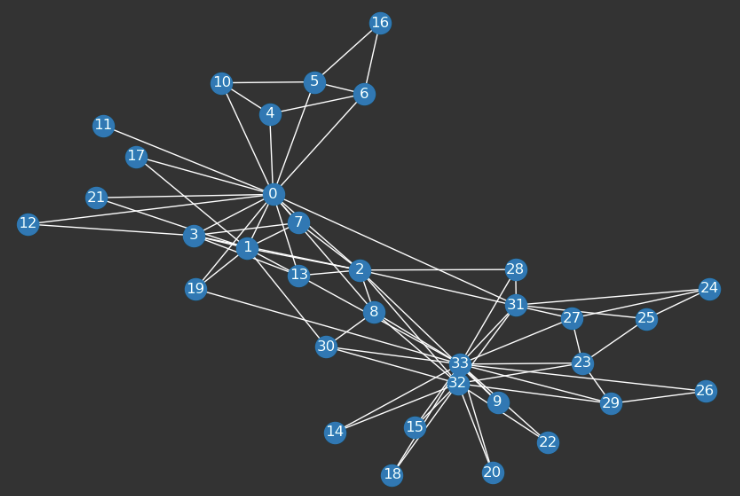
\includegraphics[width=5.9in]{./5bii.png}
            \end{minipage}
        \end{minipage}
        \newpage
        \item \begin{minipage}[t]{0.9\textwidth}
            Based purely on visuals of the graph drawing, nodes 0, 2, 33 and 32 seem to be the most
            central. Because nodes 0, 33 and 32 appear connected to so many other nodes, they likely
            have the highest degree centralities. Due to the sheer amount of connections, they likely
            fall on many shortest paths between nodes in the network also resulting in high betweenness centralities.
            Similarly, the large number of neighbours would mean there are many distences between them and other nodes
            of length 1, likely also resulting in high closeness centralities.\\
            Although node 2 doesnt seem to have a very high degree centralitiy, its placement near the center of the
            graph, almost splitting the graph evenely into two, suggests that it would have a short average distance
            to other nodes while also lying on the shortest paths between many nodes on either ends of the graph.
            These aspects suggest high closeness and betweenness centralities for node 2.
        \end{minipage}

        \item \begin{minipage}[t]{0.9\textwidth}
            \begin{minipage}[t]{0.9\textwidth}
                \vspace{0.1em} % some vertical space after the caption   
                \centering
                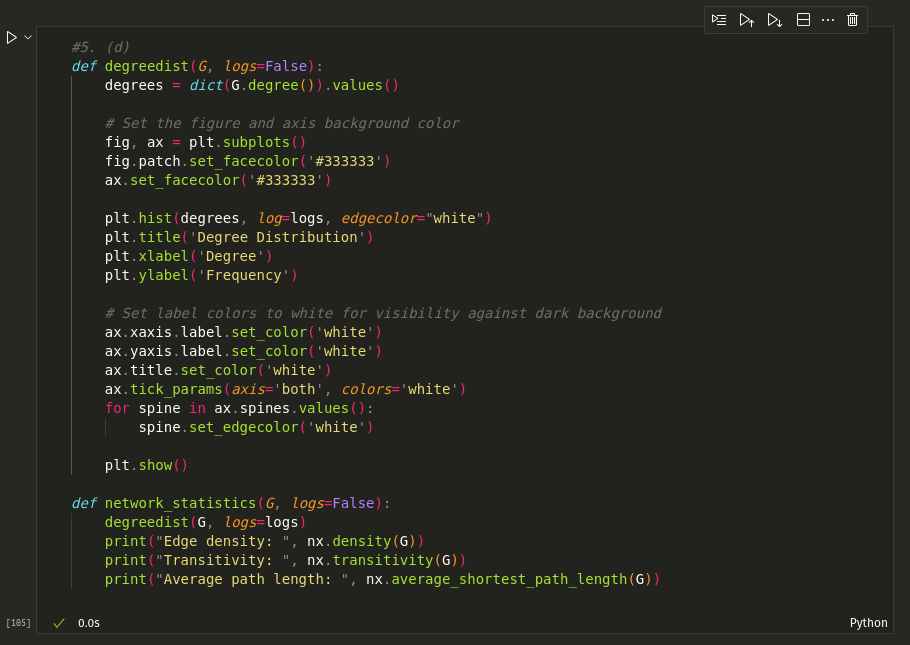
\includegraphics[width=5.9in]{./5di.png}
                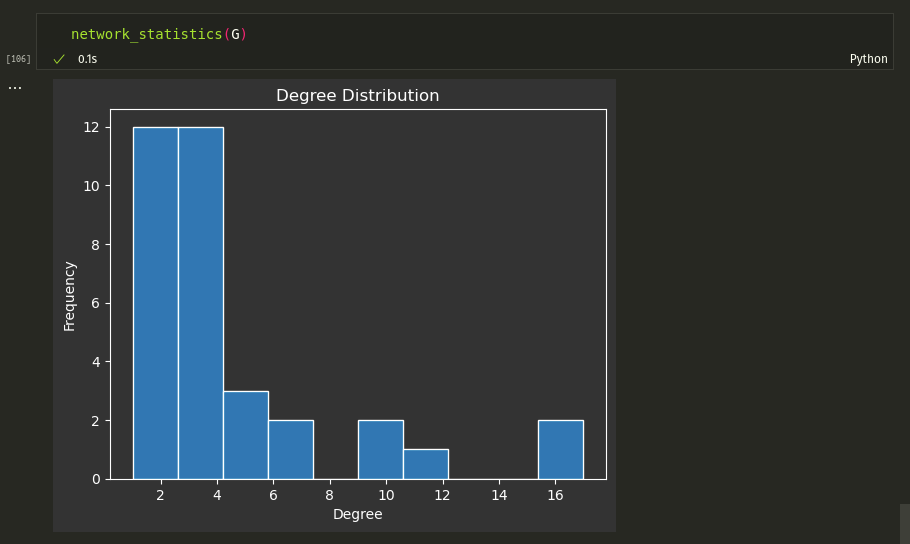
\includegraphics[width=5.9in]{./5dii.png}
            \end{minipage}
        \end{minipage}\\
        \begin{minipage}[t]{0.9\textwidth}
            \begin{minipage}[t]{0.9\textwidth}
                \centering
                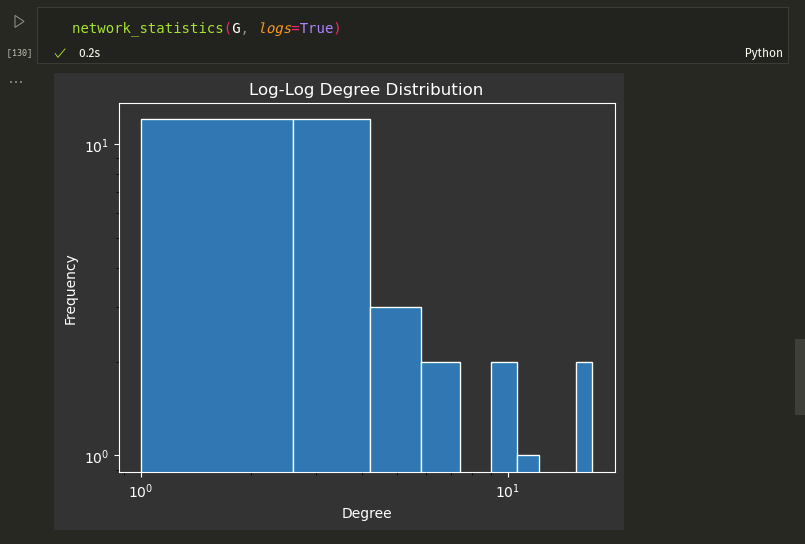
\includegraphics[width=5.9in]{./5diii.png}
            \end{minipage}
            \vspace{1em}

            From the Degree Distribution histogram we see that the majority of nodes have a
            low degree, around 2,3 and 4, while a smaller amount of nodes have higher degrees.
            This is reflected in the shape of the histogram which depicts a "long-tail" and an 
            "$L$" shape, both of which are characteristic of the power-law distribution. Although
            the log-log graph of the distribution doesnt perfectly show a linear trend, this could
            be due to the relatively small size of the network so based on initial inspection
            the degree distribution does seem to indicate a power-law.
        \end{minipage}

        \item \begin{minipage}[t]{0.9\textwidth}
        
            \begin{minipage}[t]{0.9\textwidth}
                \vspace{0.1em} % some vertical space after the caption   
                \centering
                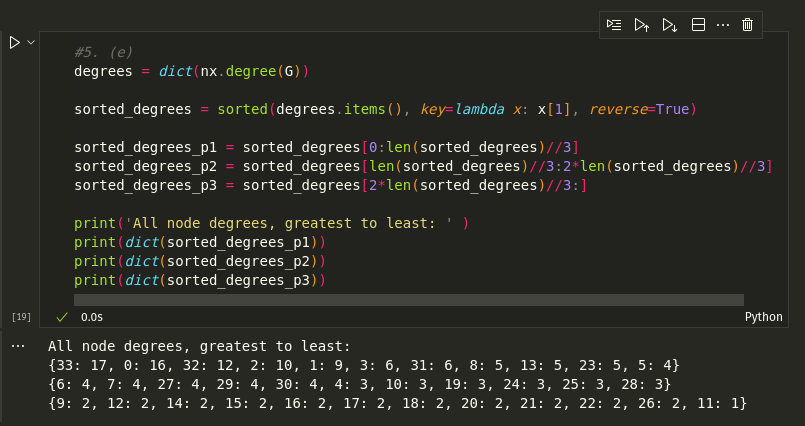
\includegraphics[width=5.9in]{./5e.png}
            \end{minipage}
        
            \vspace{1em}

            The highest degree nodes are 33, 0 and 32. In this network, connections deptict pairs
            of members that interacted outside of the karate club. We could then reasonably deduce that
            this metric indicates how interpersonally influential or involved a particular indivdual
            is in the club. A high degree individual would be someone that interactes with many
            members outside of the club indicating high sociability, multiple friendships or large
            overall influence. A low degree could indicate someone that does not have many ties to
            other memebers and so does not have much influence.

        \end{minipage}

        \item \begin{minipage}[t]{0.9\textwidth}
        
            \begin{minipage}[t]{0.9\textwidth}
                \vspace{0.1em} % some vertical space after the caption   
                \centering
                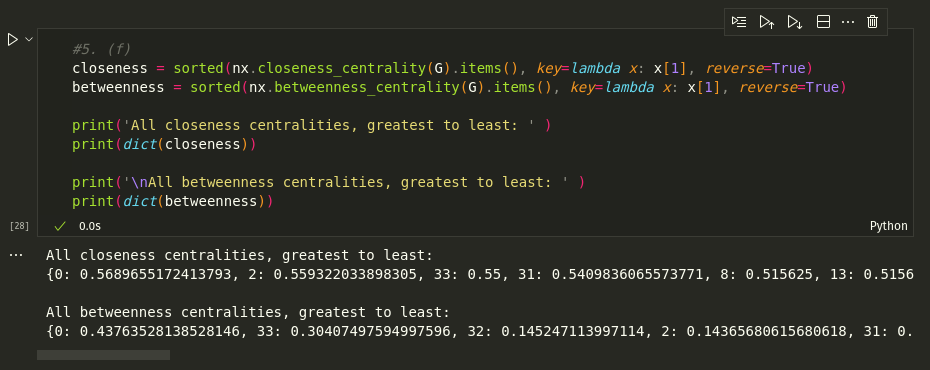
\includegraphics[width=5.9in]{./5f.png}
            \end{minipage}

        \end{minipage}

        \item \begin{minipage}[t]{0.9\textwidth}

            The three nodes with the highest closeness centrality based on the the values
            calculated above are nodes 0, 2 and 33.\\
            The three nodes with the highest betweenness centralitiy are nodes 0, 33 and 32.\\

            These rankings largely agree other than node 2 having a higher closeness centrality
            than node 33 and 32 while node 32 having a higher betweenness centrality than node 2.
            For both centrality measures, node 0 is higher than node 33 and both are among the
            top three.\\

            For the closeness centrality the node rankings make sense where 0 and 33 have
            low average distance to other nodes since they have large amounts of adjacent connections
            with distance 1. Node 2 being among the top three for this measure also make sense
            due to its placement near the ceneter of the graph resutling in a short average
            distance to other nodes on either half of the graph.\\

            For the betweeness centrality, the top three nodes are also the nodes with the top
            three degree. This also makes sense because a high number of connections to other
            nodes means that a given node likely falls on many shortest paths between other
            nodes.
        \end{minipage}

        \item \begin{minipage}[t]{0.9\textwidth}
            \textbf{(i) Coloured by Degree}\\
            \begin{minipage}[t]{0.9\textwidth}
                \vspace{0.1em} % some vertical space after the caption   
                \centering
                
\includegraphics[width=5.9in]{./5hi1.png}
                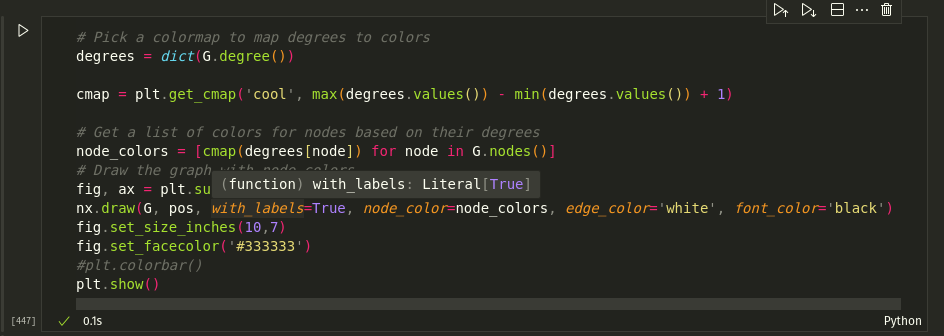
\includegraphics[width=5.9in]{./5hi2.png}
                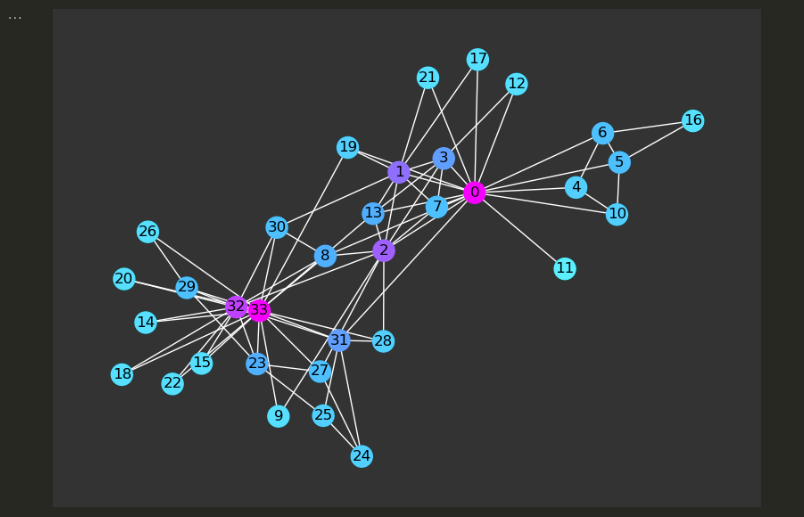
\includegraphics[width=5.9in]{./5hi3.png}
            \end{minipage}
        \end{minipage}
        \newpage
        \begin{minipage}[t]{0.9\textwidth}
                \textbf{(ii) Coloured by Closeness Centrality}\\
                \begin{minipage}[t]{0.9\textwidth}
                    \vspace{0.1em} % some vertical space after the caption   
                    \centering
                    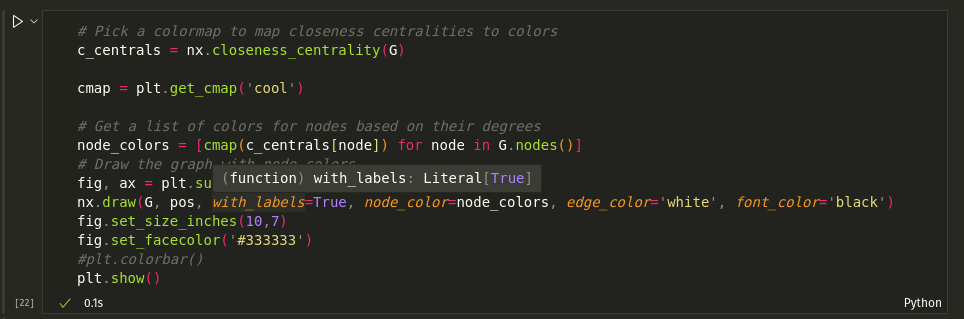
\includegraphics[width=5.9in]{./5hii1.png}
                    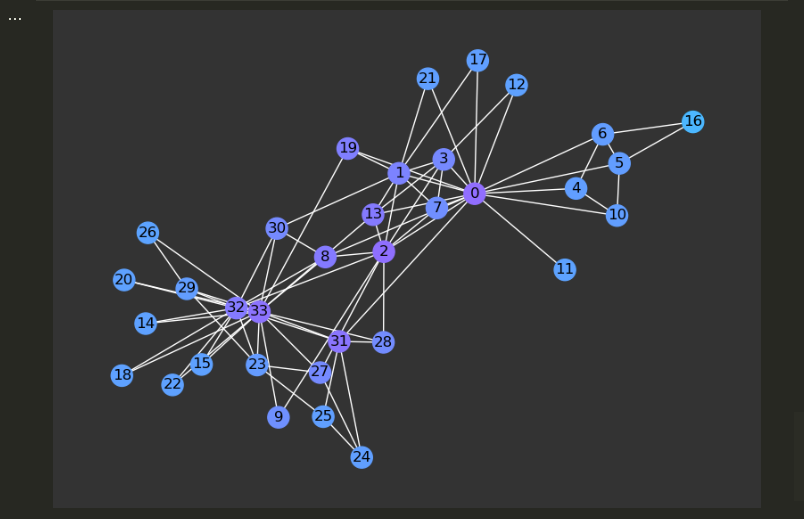
\includegraphics[width=5.9in]{./5hii2.png}
                \end{minipage}
        \end{minipage}
        \newpage
        \begin{minipage}[t]{0.9\textwidth}
                \textbf{(iii) Coloured by Betweenness Centrality}\\
                \begin{minipage}[t]{0.9\textwidth}
                    \vspace{0.1em} % some vertical space after the caption   
                    \centering
                    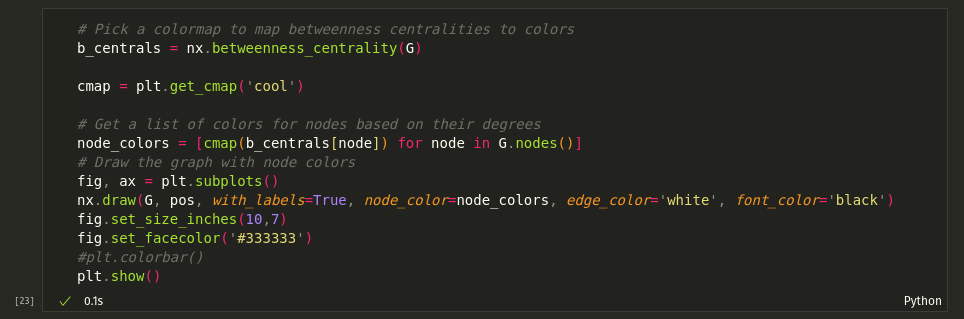
\includegraphics[width=5.9in]{./5hiii1.png}
                    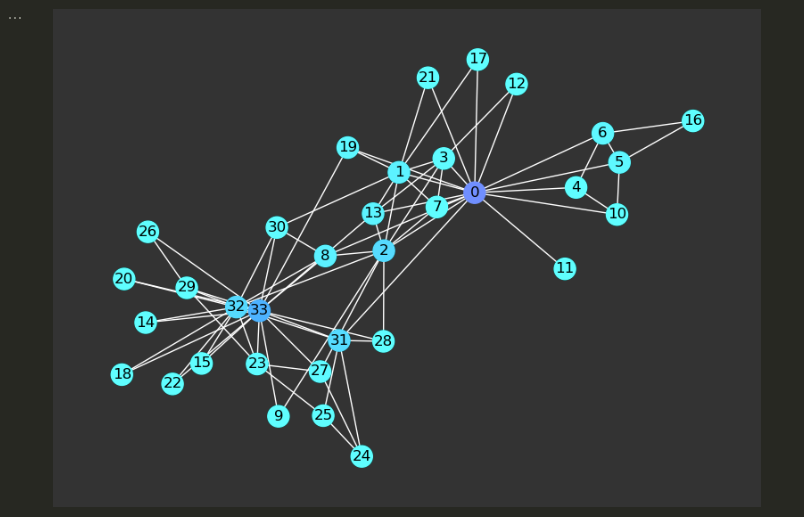
\includegraphics[width=5.9in]{./5hiii2.png}
                \end{minipage}
        \end{minipage}

        \item \begin{minipage}[t]{0.9\textwidth}
            If we are considering degree centrality as one of the centrality measures
            then this aspect would offer the greatest insight into the member playing
            the most influential role in a disagreement. It is most natural to reason
            that the members with the highest degrees are directly interacting with
            the most other members outside of the club and so will have the most
            opportunities to influence opinions. Thus, for important
            decisions and big disagreements, such memebers would cettainly hold much
            more sway than those who have a low degree centrality.\\

            If we are only considering betweenness and closeness centralities then
            a case could be made for both. We could argue that the nodes with the
            leaset average distance from all other nodes (highest closeness centrality),
            are in a position to have their message heard by the most people since they
            are the fewest interactions away from everyone else. This could play a
            large role in influcencing others.\\
            
            We could also make the point that those with the highest betweenness
            centralities have the largest amount of information flow through them
            since they stand in the way of the highest number of interaction chains
            between other memebrs. This could allow them to understand the points of
            views of many other memebera and the nuances of the disagreement better
            than most.

        \end{minipage}

    \end{enumerate}

\end{document}